\documentclass{standalone}
\usepackage{tikz}
\usetikzlibrary{patterns, positioning}


\begin{document}
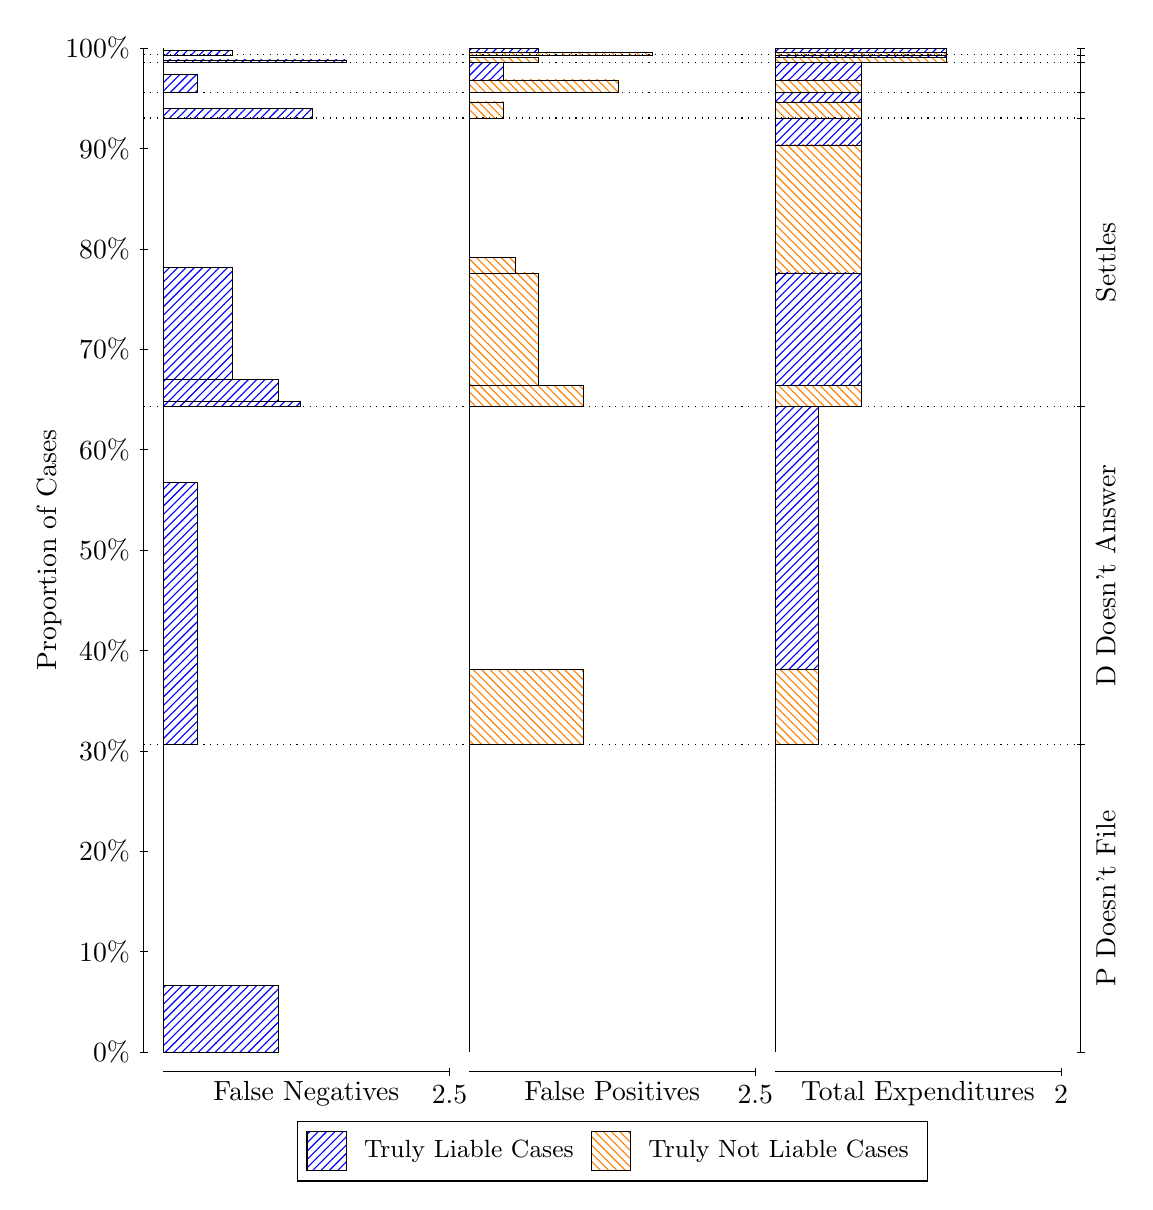
\begin{tikzpicture}
\draw[black, very thin] (1.5,1.75) -- (1.5,14.5);
\node[rotate=90, text=black, anchor=center] at (0.3, 8.125) {Proportion of Cases};
\draw[black, very thin] (1.45,1.75) -- (1.55,1.75);
\node[text=black, anchor=east] at (1.45, 1.75) {0\%};
\draw[black, very thin] (1.45,3.025) -- (1.55,3.025);
\node[text=black, anchor=east] at (1.45, 3.025) {10\%};
\draw[black, very thin] (1.45,4.3) -- (1.55,4.3);
\node[text=black, anchor=east] at (1.45, 4.3) {20\%};
\draw[black, very thin] (1.45,5.575) -- (1.55,5.575);
\node[text=black, anchor=east] at (1.45, 5.575) {30\%};
\draw[black, very thin] (1.45,6.85) -- (1.55,6.85);
\node[text=black, anchor=east] at (1.45, 6.85) {40\%};
\draw[black, very thin] (1.45,8.125) -- (1.55,8.125);
\node[text=black, anchor=east] at (1.45, 8.125) {50\%};
\draw[black, very thin] (1.45,9.4) -- (1.55,9.4);
\node[text=black, anchor=east] at (1.45, 9.4) {60\%};
\draw[black, very thin] (1.45,10.675) -- (1.55,10.675);
\node[text=black, anchor=east] at (1.45, 10.675) {70\%};
\draw[black, very thin] (1.45,11.95) -- (1.55,11.95);
\node[text=black, anchor=east] at (1.45, 11.95) {80\%};
\draw[black, very thin] (1.45,13.225) -- (1.55,13.225);
\node[text=black, anchor=east] at (1.45, 13.225) {90\%};
\draw[black, very thin] (1.45,14.5) -- (1.55,14.5);
\node[text=black, anchor=east] at (1.45, 14.5) {100\%};

\draw[black, very thin] (13.4,1.75) -- (13.4,14.5);
\draw[black, very thin] (13.35,1.75) -- (13.45,1.75);
\node[anchor=west] at (13.35, 1.75) {};
\draw[black, very thin] (13.35,5.6541) -- (13.45,5.6541);
\node[anchor=west] at (13.35, 5.6541) {};
\draw[black, very thin] (13.35,9.9452) -- (13.45,9.9452);
\node[anchor=west] at (13.35, 9.9452) {};
\draw[black, very thin] (13.35,13.612) -- (13.45,13.612);
\node[anchor=west] at (13.35, 13.612) {};
\draw[black, very thin] (13.35,13.939) -- (13.45,13.939);
\node[anchor=west] at (13.35, 13.939) {};
\draw[black, very thin] (13.35,14.319) -- (13.45,14.319);
\node[anchor=west] at (13.35, 14.319) {};
\draw[black, very thin] (13.35,14.413) -- (13.45,14.413);
\node[anchor=west] at (13.35, 14.413) {};
\draw[black, very thin] (13.35,14.5) -- (13.45,14.5);
\node[anchor=west] at (13.35, 14.5) {};

\draw[black, very thin, pattern color=blue, pattern=north east lines] (1.75,1.75) rectangle (3.2033,2.5915);
\draw[black, very thin, pattern color=orange, pattern=north west lines] (1.75,2.5915) rectangle (1.75,5.6541);
\draw[black, very thin, pattern color=blue, pattern=north east lines] (1.75,5.6541) rectangle (2.186,8.9861);
\draw[black, very thin, pattern color=orange, pattern=north west lines] (1.75,8.9861) rectangle (1.75,9.9452);
\draw[black, very thin, pattern color=blue, pattern=north east lines] (1.75,9.9452) rectangle (3.494,10.014);
\draw[black, very thin, pattern color=blue, pattern=north east lines] (1.75,10.014) rectangle (3.2033,10.289);
\draw[black, very thin, pattern color=blue, pattern=north east lines] (1.75,10.289) rectangle (2.622,11.715);
\draw[black, very thin, pattern color=orange, pattern=north west lines] (1.75,11.715) rectangle (1.75,13.612);
\draw[black, very thin, pattern color=blue, pattern=north east lines] (1.75,13.612) rectangle (3.6393,13.734);
\draw[black, very thin, pattern color=orange, pattern=north west lines] (1.75,13.734) rectangle (1.75,13.939);
\draw[black, very thin, pattern color=blue, pattern=north east lines] (1.75,13.939) rectangle (2.186,14.162);
\draw[black, very thin, pattern color=orange, pattern=north west lines] (1.75,14.162) rectangle (1.75,14.319);
\draw[black, very thin, pattern color=blue, pattern=north east lines] (1.75,14.319) rectangle (4.0753,14.348);
\draw[black, very thin, pattern color=orange, pattern=north west lines] (1.75,14.348) rectangle (1.75,14.413);
\draw[black, very thin, pattern color=blue, pattern=north east lines] (1.75,14.413) rectangle (2.622,14.471);
\draw[black, very thin, pattern color=orange, pattern=north west lines] (1.75,14.471) rectangle (1.75,14.5);
\draw[black, very thin, pattern color=orange, pattern=north west lines] (5.6333,1.75) rectangle (5.6333,4.8125);
\draw[black, very thin, pattern color=blue, pattern=north east lines] (5.6333,4.8125) rectangle (5.6333,5.6541);
\draw[black, very thin, pattern color=orange, pattern=north west lines] (5.6333,5.6541) rectangle (7.0867,6.6131);
\draw[black, very thin, pattern color=blue, pattern=north east lines] (5.6333,6.6131) rectangle (5.6333,9.9452);
\draw[black, very thin, pattern color=orange, pattern=north west lines] (5.6333,9.9452) rectangle (7.0867,10.219);
\draw[black, very thin, pattern color=orange, pattern=north west lines] (5.6333,10.219) rectangle (6.5053,11.645);
\draw[black, very thin, pattern color=orange, pattern=north west lines] (5.6333,11.645) rectangle (6.2147,11.843);
\draw[black, very thin, pattern color=blue, pattern=north east lines] (5.6333,11.843) rectangle (5.6333,13.612);
\draw[black, very thin, pattern color=orange, pattern=north west lines] (5.6333,13.612) rectangle (6.0693,13.817);
\draw[black, very thin, pattern color=blue, pattern=north east lines] (5.6333,13.817) rectangle (5.6333,13.939);
\draw[black, very thin, pattern color=orange, pattern=north west lines] (5.6333,13.939) rectangle (7.5227,14.095);
\draw[black, very thin, pattern color=blue, pattern=north east lines] (5.6333,14.095) rectangle (6.0693,14.319);
\draw[black, very thin, pattern color=orange, pattern=north west lines] (5.6333,14.319) rectangle (6.5053,14.384);
\draw[black, very thin, pattern color=blue, pattern=north east lines] (5.6333,14.384) rectangle (5.6333,14.413);
\draw[black, very thin, pattern color=orange, pattern=north west lines] (5.6333,14.413) rectangle (7.9587,14.442);
\draw[black, very thin, pattern color=blue, pattern=north east lines] (5.6333,14.442) rectangle (6.5053,14.5);
\draw[black, very thin, pattern color=orange, pattern=north west lines] (9.5167,1.75) rectangle (9.5167,4.8125);
\draw[black, very thin, pattern color=blue, pattern=north east lines] (9.5167,4.8125) rectangle (9.5167,5.6541);
\draw[black, very thin, pattern color=orange, pattern=north west lines] (9.5167,5.6541) rectangle (10.062,6.6131);
\draw[black, very thin, pattern color=blue, pattern=north east lines] (9.5167,6.6131) rectangle (10.062,9.9452);
\draw[black, very thin, pattern color=orange, pattern=north west lines] (9.5167,9.9452) rectangle (10.607,10.219);
\draw[black, very thin, pattern color=blue, pattern=north east lines] (9.5167,10.219) rectangle (10.607,11.645);
\draw[black, very thin, pattern color=orange, pattern=north west lines] (9.5167,11.645) rectangle (10.607,13.269);
\draw[black, very thin, pattern color=blue, pattern=north east lines] (9.5167,13.269) rectangle (10.607,13.612);
\draw[black, very thin, pattern color=orange, pattern=north west lines] (9.5167,13.612) rectangle (10.607,13.817);
\draw[black, very thin, pattern color=blue, pattern=north east lines] (9.5167,13.817) rectangle (10.607,13.939);
\draw[black, very thin, pattern color=orange, pattern=north west lines] (9.5167,13.939) rectangle (10.607,14.095);
\draw[black, very thin, pattern color=blue, pattern=north east lines] (9.5167,14.095) rectangle (10.607,14.319);
\draw[black, very thin, pattern color=orange, pattern=north west lines] (9.5167,14.319) rectangle (11.697,14.384);
\draw[black, very thin, pattern color=blue, pattern=north east lines] (9.5167,14.384) rectangle (11.697,14.413);
\draw[black, very thin, pattern color=orange, pattern=north west lines] (9.5167,14.413) rectangle (11.697,14.442);
\draw[black, very thin, pattern color=blue, pattern=north east lines] (9.5167,14.442) rectangle (11.697,14.5);
\draw[black, dotted] (1.5,5.6541) -- (13.4,5.6541);
\draw[black, dotted] (1.5,9.9452) -- (13.4,9.9452);
\draw[black, dotted] (1.5,13.612) -- (13.4,13.612);
\draw[black, dotted] (1.5,13.939) -- (13.4,13.939);
\draw[black, dotted] (1.5,14.319) -- (13.4,14.319);
\draw[black, dotted] (1.5,14.413) -- (13.4,14.413);
\draw[black, very thin] (1.75,1.5) -- (5.3833,1.5);
\node[text=black, anchor=north] at (3.5667, 1.5) {False Negatives};
\draw[black, very thin] (5.3833,1.45) -- (5.3833,1.55);
\node[text=black, anchor=north] at (5.3833, 1.45) {2.5};

\draw[black, very thin] (5.6333,1.5) -- (9.2667,1.5);
\node[text=black, anchor=north] at (7.45, 1.5) {False Positives};
\draw[black, very thin] (9.2667,1.45) -- (9.2667,1.55);
\node[text=black, anchor=north] at (9.2667, 1.45) {2.5};

\draw[black, very thin] (9.5167,1.5) -- (13.15,1.5);
\node[text=black, anchor=north] at (11.333, 1.5) {Total Expenditures};
\draw[black, very thin] (13.15,1.45) -- (13.15,1.55);
\node[text=black, anchor=north] at (13.15, 1.45) {2};

\node[text=black, centered, rotate=90] at (13.72, 3.702) {P Doesn't File};
\node[text=black, centered, rotate=90] at (13.72, 7.7996) {D Doesn't Answer};
\node[text=black, centered, rotate=90] at (13.72, 11.779) {Settles};





\draw (7.449999999999999,1.5) node[draw=none] (baseCoordinate) {};
\begin{scope}[align=center]
        \matrix[scale=0.5, draw=black, below=0.5cm of baseCoordinate, nodes={draw}, column sep=0.1cm]{
            \node[rectangle, draw, minimum width=0.5cm, minimum height=0.5cm, pattern color=blue, pattern=north east lines] {}; &
            \node[draw=none, font=\small, text=black] (B) {Truly Liable Cases}; &
            \node[rectangle, draw, minimum width=0.5cm, minimum height=0.5cm, pattern color=orange, pattern=north west lines] {}; &
            \node[draw=none, font=\small, text=black] (B) {Truly Not Liable Cases}; \\
            };
\end{scope}

\end{tikzpicture}
\end{document}